% ==============================================================================
% PG - Sophie Dilhon
% Capítulo 3 - Especificação de Requisitos
% ==============================================================================
\chapter{Especificação de Requisitos}
\label{chap-especificacao-requisitos}

Este capítulo tem como objetivo apresentar a especificação de requisitos do SCAP (Sistema de Controle de Afastamento de Professores), 
assim como os modelos de casos de uso levantados por \citeonline{duarte:2014} e \citeonline{prado:2015}, que serão utilizados como base para a implementação do sistema.

\section{Descrição do Escopo}
\label{sec-espec-escopo}
O SCAP é um sistema que visa auxiliar o gerenciamento das solicitações de
afastamento de professores do Departamento de Informática (DI) da Universidade Federal do Espírito Santo (UFES)
para participação em eventos, sejam eles no Brasil ou no exterior. 
Nesses casos, o professor deve submeter uma solicitação de afastamento temporário
que será avaliada pelos professores do DI, e em alguns casos,
pela reitoria do Centro Tecnológico (CT) e Pró-Reitoria de Pesquisa e Pós-Graduação (PRPPG) da UFES.
Ao ser aprovada em todas as instâncias, o afastamento temporário é autorizado.

Para eventos no Brasil, as solicitações tramitam apenas no DI, e devem ser
aprovadas pela Câmara Departamental (formada pelos funcionários do Departamento
e representantes discentes). Dessa forma, o professor envia seu pedido para a
lista de e-mails dos funcionários do DI, endereçado ao Chefe de Departamento,
cargo exercido temporariamente por um professores do DI. Caso nenhum membro
da Câmara Departamental se oponha ao pedido em até dez dias, o afastamento é autorizado.

Para eventos no exterior, um professor, que não tenha parentesco com o solicitante,
é escolhido para ser o relator do pedido. Após emitido o parecer do relator, o
processo deve ser aprovado pela Câmara Departamental, como no caso de eventos no Brasil.
Além disso, a solicitação deve ser aprovada pela reitoria do CT e PRPPG.
Depois de ser aprovado por todos os envolvidos, o afastamento é autorizado
e o pedido é publicado no Diário Oficial da União. 
No entanto, o SCAP é responsável por assistir o processo apenas dentro do DI,
não havendo uma integração com os processos da reitoria do CT e PRPPG.

O objetivo do SCAP é agilizar e simplificar o processo para os professores
e secretários do DI, automatizando o envio de e-mails aos membros envolvidos
e utilizando formulários para a criação dos documentos necessários.


\section{Modelos de Casos de Uso}
\label{sec-espec-casos-uso}

Na tabela~\ref{tab:atores} são apresentados os atores do SCAP, identificados
por \citeonline{duarte:2014} no levantamento de requisitos do sistema.

\begin{table}[h!]
    \centering
    \caption{Atores do Sistema}
    \label{tab:atores}
    \begin{tabular}{|p{5cm}|p{10cm}|}
    \hline
    \textbf{Atores} & \textbf{Descrição}\\ \hline
    Professor & Professor efetivo do DI \\ \hline
    Secretário & Secretário do DI \\ \hline
    Chefe de Departamento & Professor do DI que está realizando a função administrativa de chefe ou subchefe do departamento  \\ \hline
    \end{tabular}
\end{table}

O secretário é responsável pela administração do sistema. Sendo assim,
ele deve cadastrar os professores, e seus parentescos, além dos mandatos
de chefes e subchefes do departamento. Outras tarefas incluem, cadastrar
as decisões do CT e PRPPG (em casos de eventos no exterior), e arquivar
processos que forem concluídos.

O professor pode cadastrar solicitações de afastamento e também se manifestar
contra pedidos de outros professores, caso esteja dentro do prazo para tal.
Se for adicionado como relator de um pedido de afastamento no exterior,
o professor deve emitir um parecer sobre o mesmo, e assim decidir se o
DI aprova ou não tal solicitação.

O chefe de departamento é um professor que foi eleito para exercer a função
administrativa durante um período de tempo. Assim, além das funcionalidades
comuns a um professor, ele também é responsável por nomear relatores
para pedidos de afastamento no exterior.


O SCAP foi dividido em dois módulos: Cadastral e Núcleo. O primeiro é responsável pela parte
cadastral, ou seja, casos de uso dos secretários. Já o segundo, abrange
as funcionalidades de professores e chefes de departamento. Uma versão mais
completa e detalhada pode ser vista em~\cite{duarte:2014,prado:2015}.
As Figuras~\ref{fig:casos-de-uso-cadastral} e~\ref{fig:casos-de-uso-nucleo} apresentam
os diagramas de casos de uso do SCAP.

\begin{figure}
    \centering
    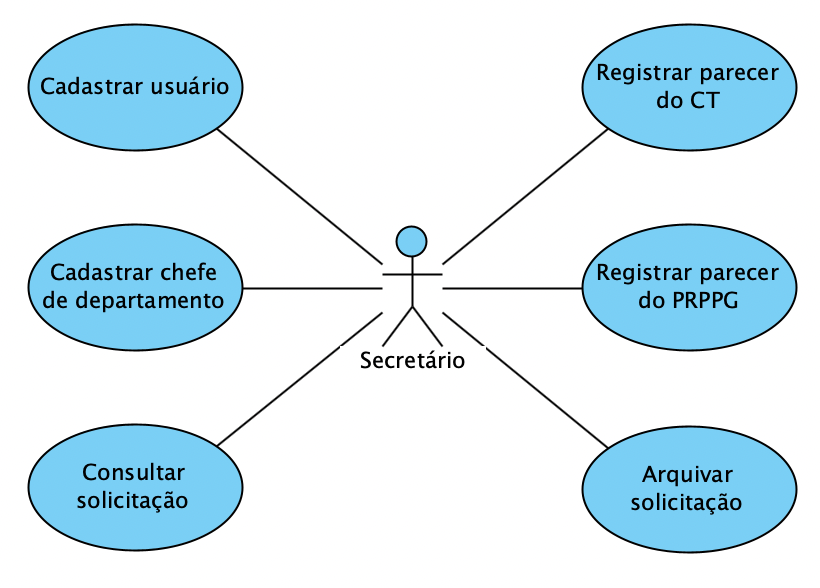
\includegraphics[width=0.6\textwidth]{figuras/fig-caso-cadastral.png}
    \caption{Diagrama de Casos de Uso do subsistema Cadastral~\cite{prado:2015}.}
    \label{fig:casos-de-uso-cadastral}
\end{figure}

Em \textbf{Cadastrar Usuário}, o secretário cadastra um novo usuário no sistema, sendo
este um professor ou um secretário, junto de seus dados. Já em \textbf{Cadastrar chefe de departamento},
o secretário cadastra o mandato do chefe ou subchefe do departamento, assim como suas datas de início e fim.

Os casos de uso \textbf{Registrar parecer do PRPPG} e \textbf{Registrar parecer do CT}, ocorrem
apenas em casos de afastamento no exterior. O secretário é responsável por registrar as decisões
do PRPPG e CT, respectivamente, quando estes aprovam ou não um pedido de afastamento.

Em \textbf{Arquivar solicitação}, o secretário arquiva um processo que foi concluído, ou seja, que
já passou por todas as instâncias e foi aprovado. \textbf{Consultar Solicitação} é um caso de uso
comum aos professores e secretários, e permite que o usuário consulte o andamento e os dados de um
pedido de afastamento.


\begin{figure}
    \centering
    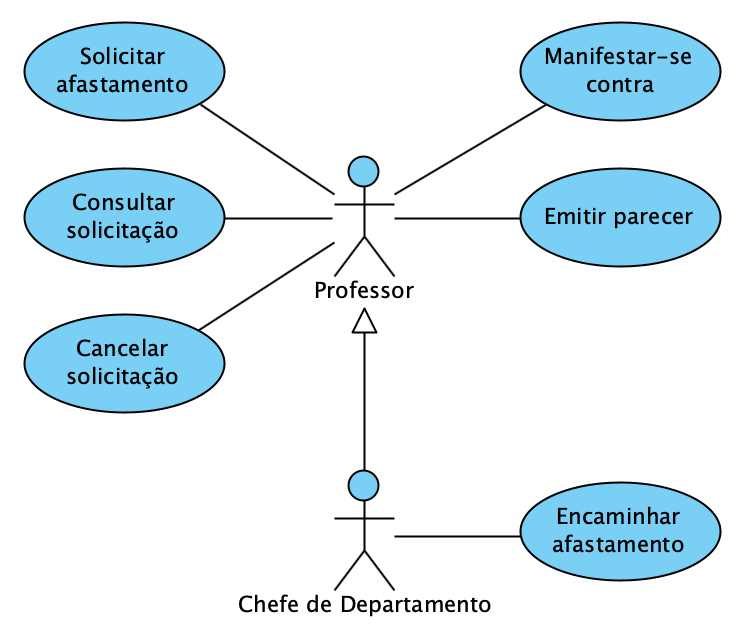
\includegraphics[width=0.6\textwidth]{figuras/fig-caso-nucleo.png}
    \caption{Diagrama de Casos de Uso do subsistema Núcleo~\cite{prado:2015}.}
    \label{fig:casos-de-uso-nucleo}
\end{figure}


O caso de uso \textbf{Solicitar afastamento} é o principal caso de uso do sistema, e permite
que um professor solicite um afastamento para participar de um evento. Para isso devem ser informadas
as datas de início e fim, o nome do evento e se este é nacional ou internacional. 
Enquanto em \textbf{Cancelar solicitação}, o professor pode cancelar um pedido feito por ele próprio,
alterando assim o estado do processo para cancelado.

O professor pode ainda \textbf{Manifestar-se contra} um pedido de afastamento de 
outro professor, caso esteja dentro do prazo para tal, registrando o motivo de sua opinião.
Uma reunião deve então ser agendada para que os professores decidam se o afastamento será aprovado ou não.
Por último, \textbf{Emitir parecer} é um caso de uso exclusivo de professores que foram nomeados
como relator de um pedido de afastamento no exterior. O professor deve cadastrar um parecer sobre a solicitação.

O chefe de departamento, além das funcionalidades comuns a um professor, também pode \textbf{Encaminhar afastamento},
ou seja, indicar um professor como relator para um pedido de afastamento no exterior. 


\section{Análise do SCAP}
\label{sec-espec-analise-scap}

A Figura~\ref{fig:diagrama-classes} apresenta o diagrama de classes do SCAP, adaptado
do levantamento feito por~\citeonline{prado:2015}, juntamente com o que havia sido
levantado anteriormente por~\citeonline{duarte:2014}.

\begin{figure}
    \centering  
    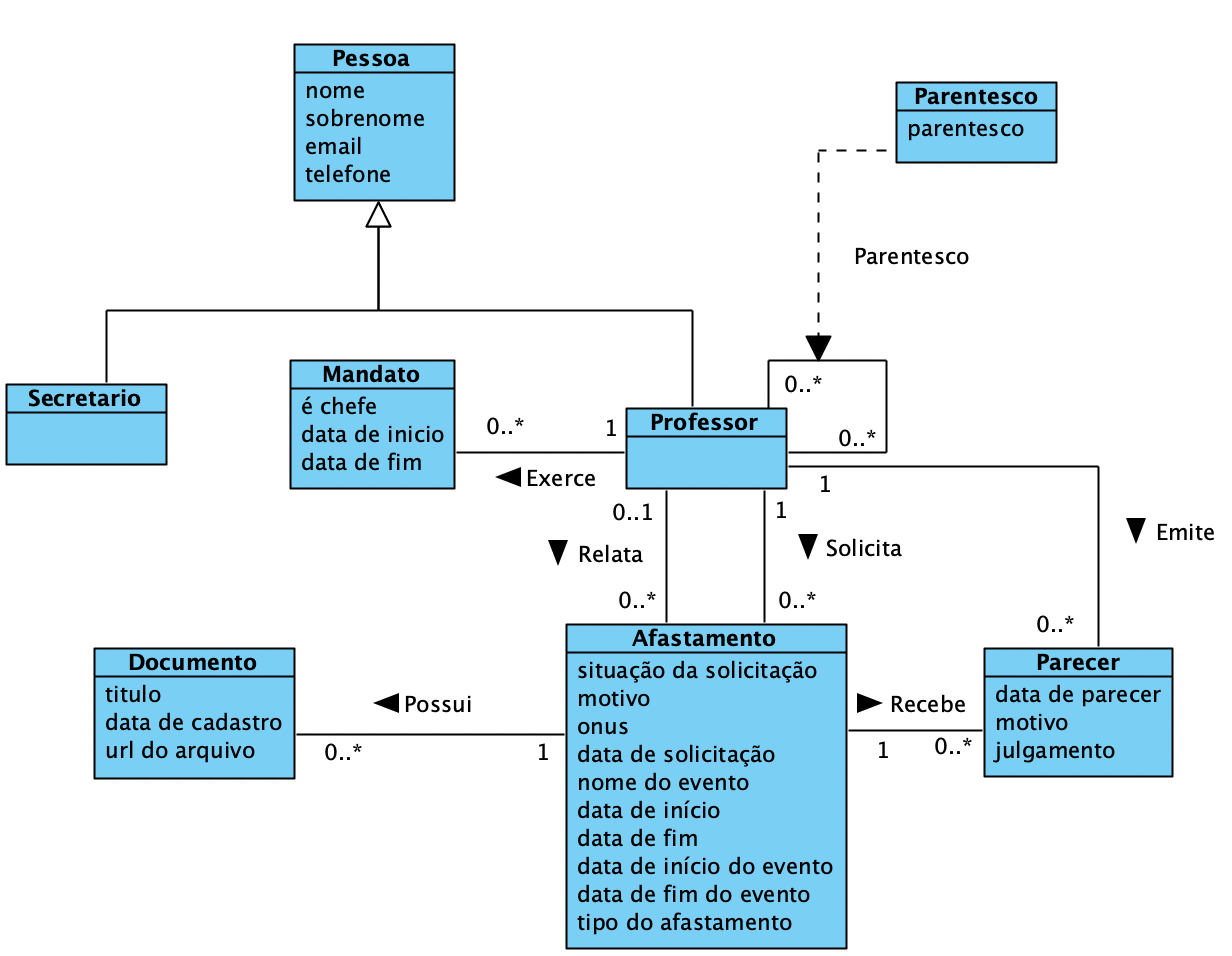
\includegraphics[width=0.9\textwidth]{figuras/fig-diagrama-classes.png}
    \caption{Diagrama de Classes do SCAP.}
    \label{fig:diagrama-classes}
\end{figure}

As classes \textbf{Professor} e \textbf{Secretario} representam os professores
e secretários do DI, respectivamente, ambas herdam as propriedades da classe \textbf{Pessoa},
que contém as informações pessoais do usuário. A classe \textbf{Parentesco} 
guarda relações de parentesco que podem existir entre professores do DI.
A classe \textbf{Mandato} representa o tempo do mandato, de chefe ou subchefe do departamento,
que o professor está exercendo.

A classe \textbf{Afastamento} guarda informações sobre os pedidos de afastamento
feitos pelos professores, como as datas de início e fim, o nome do evento e etc.
Este pode ou não possuir um \textbf{Documento} associado, e deve possuir um \textbf{Relator}
caso seja um pedido de afastamento no exterior. Um professor pode ser relator de vários afastamentos,
mas seu \textbf{Parecer} é único para cada solicitação de afastamento internacional.


Restrições de integridade complementam o modelos de classes, que por muitas vezes não são
capazes de representá-las por notações gráficas. Abaixo estão listadas as restrições
levantadas por~\citeonline{duarte:2014} e posteriormente ampliadas por~\citeonline{prado:2015}.

\begin{itemize}
    \item Um professor não pode ser nomeado como relator, nem emitir um parecer, para sua própria solicitação de afastamento;
    \item Um professor não pode ser relator de um afastamento solicitado por um parente.
    \item A data de início de um afastamento não pode ser posterior a data de fim do mesmo afastamento;
    \item A data de início de um mandato de professor não pode ser posterior a data de fim do mesmo mandato;
    \item Não pode haver mais de dois professores (chefe e subchefe de departamento) exercendo um mandato ao mesmo tempo;
    \item O secretário do departamento não pode abrir uma solicitação de afastamento;
    
\end{itemize}